\chapter{自由 Schrödinger 方程}\label{chap:free-schrodinger}

本章考察一维自由 Schrödinger 方程的各种求解方法.这里“自由”意味着没有力作用在粒子上,因此可以取势能 \(V\) 恒等于零.于是自由 Schrödinger 方程为
\begin{equation}
\frac{\partial\psi}{\partial t}
=\frac{i\hbar}{2m}\frac{\partial^{2}\psi}{\partial x^{2}},
\label{eq:free-schrodinger}
\end{equation}
并带有形如
\[
\psi(x,0)=\psi_{0}(x)
\]
的初始条件.我们将识别这个方程解的一些关键特征,例如“波包的扩散”以及“相速度”和“群速度”的区别.特别地,群速度的概念将证实我们的预期:动量为 \(p\) 的粒子应以速度 \(v=p/m\) 运动.

在尝试求解自由 Schrödinger 方程之前,先观察位置和动量期望值的时间演化.如果把命题~\ref{prop:expected-position-momentum} 应用于 \(V\) 恒等于零的情形,就有
\[
\frac{\mathrm{d}}{\mathrm{d}t}\langle X\rangle_{\psi(t)}
=\frac{1}{m}\langle P\rangle_{\psi(t)},
\qquad
\frac{\mathrm{d}}{\mathrm{d}t}\langle P\rangle_{\psi(t)}=0.
\]
因此,\(\langle P\rangle_{\psi(t)}\) 与时间无关,从而 \(\langle X\rangle_{\psi(t)}\) 关于时间是线性的:
\[
\langle X\rangle_{\psi(t)}
=\langle X\rangle_{\psi_{0}}+\frac{t}{m}\langle P\rangle_{\psi_{0}},
\qquad
\langle P\rangle_{\psi(t)}=\langle P\rangle_{\psi_{0}}.
\]
所以,自由 Schrödinger 方程是期望位置和期望动量严格沿经典轨迹演化的特殊情形之一;当 \(V\equiv0\) 时,这些经典轨迹尤其简单.

\section{用 Fourier 变换求解}\label{sec:free-fourier}

我们寻找 \(\mathbb{R}^{1}\) 上自由 Schrödinger 方程的形如
\begin{equation}
\psi(x,t)=e^{i(kx-\omega(k)t)}
\label{eq:free-plane-wave}
\end{equation}
的解,其中 \(k\) 是空间频率,而 \(\omega(k)\) 是尚未确定的时间频率.这样的解对固定 \(t\) 关于 \(x\) 并不平方可积,不过我们最终会回到平方可积解.将式~\eqref{eq:free-plane-wave} 代入式~\eqref{eq:free-schrodinger},立即得到
\begin{equation}
\omega(k)=\frac{\hbar k^{2}}{2m}.
\label{eq:free-dispersion}
\end{equation}
把偏微分方程某个解中的时间频率 \(\omega\) 表示为空间频率 \(k\) 的函数,这样的公式称为\emph{色散关系}.

注意,式~\eqref{eq:free-plane-wave} 可以写成
\[
\psi(x,t)=\exp\left(ik\left(x-\frac{\omega(k)}{k}t\right)\right).
\]
把函数 \(f(x)\) 替换成 \(f(x-a)\),其效果是把 \(f\) 向右平移 \(a\).因此,时间演化的效果是把初始函数向右平移 \((\omega(k)/k)t\).这意味着 \(\psi(x,t)\) 以速度 \(\omega(k)/k\) 向右运动.由于第~\ref{sec:wave-packet-first} 节中的原因,这个速度称为相速度.

相速度是自由 Schrödinger 方程的纯指数解传播的速度.计算得
\[
\frac{\omega(k)}{k}=\frac{\hbar k}{2m}.
\]
我们已经说过,形如 \(e^{ikx}\) 的波函数表示动量 \(p=\hbar k\) 的粒子.于是得到如下有些奇怪的结论.

\begin{proposition}[相速度]\label{prop:phase-velocity}
动量为 \(p=\hbar k\) 的粒子的相速度为
\[
\text{相速度}=\frac{\omega(k)}{k}
=\frac{\hbar k}{2m}
=\frac{p}{2m}.
\]
这个速度是动量为 \(p\) 的经典粒子速度的一半.
\end{proposition}

命题~\ref{prop:phase-velocity} 可能让我们以为基本关系 \(p=\hbar k\) 少了一个因子 \(2\).不过,我们将看到,相速度——纯指数解的速度——不是动量为 \(p\) 的粒子的“真实”速度.真实速度是“群速度”,它最终会如预期一样等于 \(p/m\).

暂时先不讨论速度问题,下面用式~\eqref{eq:free-plane-wave} 形式的解构造一般解.利用附录~\ref{app:subsec:fourier-transform} 中讨论的 Fourier 变换,可以把自由 Schrödinger 方程的解(对“良好”的初始条件)表示为这些纯指数解的“叠加”.

\begin{proposition}[Fourier 表示的自由演化]\label{prop:free-fourier-solution}
设 \(\psi_{0}\) 是一个“良好”的函数,例如 Schwartz 函数(定义~\ref{app:def:schwartz}).记 \(\psi_{0}\) 的 Fourier 变换为 \(\widehat{\psi}_{0}\),并令
\begin{equation}
\psi(x,t)=\frac{1}{\sqrt{2\pi}}\int_{-\infty}^{\infty}
\widehat{\psi}_{0}(k)e^{i(kx-\omega(k)t)}\,\mathrm{d}k,
\label{eq:free-fourier-solution}
\end{equation}
其中 \(\omega(k)\) 由式~\eqref{eq:free-dispersion} 定义.那么 \(\psi(x,t)\) 是以 \(\psi_{0}\) 为初始条件的自由 Schrödinger 方程的解.
\end{proposition}

\begin{proof}
Schwartz 函数的 Fourier 变换仍是 Schwartz 函数,因此当 \(k\to\pm\infty\) 时,\(\widehat{\psi}_{0}(k)\) 比 \(1/k^{4}\) 衰减得更快.另一方面,对函数 \(e^{ikx}\) 的导数积分可得估计
\[
\left|\frac{e^{ik(x+h)}-e^{ikx}}{h}\right|\le |k|.
\]
于是可以使用 \(|k|\,|\widehat{\psi}_{0}(k)|\) 作为控制函数并应用控制收敛定理,把关于 \(x\) 的导数移入式~\eqref{eq:free-fourier-solution} 的积分号内;该导数会在积分中带下来一个因子 \(ik\).\(\widehat{\psi}_{0}\) 的衰减允许我们重复这个论证,把二阶导数也移入积分号内.类似地,也可以把关于 \(t\) 的导数移入积分号内.

对每个固定的 \(k\),\(\exp(i(kx-\omega(k)t))\) 都满足 Schrödinger 方程,因此在积分号下求导说明 \(\psi(x,t)\) 也满足 Schrödinger 方程.Fourier 反演公式给出 \(\psi(x,0)=\psi_{0}(x)\).
\end{proof}

\begin{proposition}[自由演化的 Fourier 变换]\label{prop:free-fourier-transform}
若 \(\psi(x,t)\) 如命题~\ref{prop:free-fourier-solution},则固定 \(t\) 关于 \(x\) 的 Fourier 变换为
\begin{equation}
\widehat{\psi}(k,t)
=\widehat{\psi}_{0}(k)\exp\left(-i\frac{\hbar k^{2}}{2m}t\right).
\label{eq:free-fourier-time}
\end{equation}
\end{proposition}

\begin{proof}
把式~\eqref{eq:free-fourier-solution} 写成
\[
\psi(x,t)=\frac{1}{\sqrt{2\pi}}\int_{-\infty}^{\infty}
e^{ikx}\widehat{\psi}_{0}(k)e^{-i\omega(k)t}\,\mathrm{d}k.
\]
由 Fourier 分解的唯一性(即逆 Fourier 变换的单射性,而这来自 Plancherel 公式),\(\psi(x,t)\) 的 Fourier 变换必为方括号中的函数.代入 \(\omega(k)\) 的表达式~\eqref{eq:free-dispersion},即可得到所需结果.
\end{proof}

Fourier 变换是从 \(L^{2}(\mathbb{R})\) 到 \(L^{2}(\mathbb{R})\) 的酉映射.因此对任意 \(\psi_{0}\in L^{2}(\mathbb{R})\),\(\widehat{\psi}_{0}\) 也属于 \(L^{2}(\mathbb{R})\).式~\eqref{eq:free-fourier-time} 中乘在 \(\widehat{\psi}_{0}(k)\) 前的量绝对值为 \(1\),所以对任意 \(\psi_{0}\in L^{2}(\mathbb{R})\),式~\eqref{eq:free-fourier-time} 右端都是定义良好的平方可积函数,并且有定义良好的 \(L^{2}\) 逆 Fourier 变换.

\begin{definition}[自由方程的 \(L^{2}\) 时间演化]\label{def:free-l2-evolution}
对任意 \(\psi_{0}\in L^{2}(\mathbb{R})\) 和 \(t\in\mathbb{R}\),定义 \(\psi(x,t)\) 为 \(L^{2}(\mathbb{R})\) 中唯一的元素,使其关于 \(x\) 的 Fourier 变换由式~\eqref{eq:free-fourier-time} 给出.
\end{definition}

定义~\ref{def:free-l2-evolution} 为任意 \(L^{2}\) 初始条件定义了时间演化.不过,对于一般的 \(\psi_{0}\in L^{2}(\mathbb{R})\),\(\psi(x,t)\) 可能不满足经典的逐点 Schrödinger 方程,因为它可能关于 \(x\) 或 \(t\) 不可微.尽管如此,按定义~\ref{def:free-l2-evolution} 得到的 \(\psi(x,t)\) 总是在弱(分布)意义下满足 Schrödinger 方程.见练习~\ref{ex:free-weak-solution}.

\section{作为卷积的解}\label{sec:free-convolution}

根据命题~\ref{prop:free-fourier-transform},时刻 \(t\) 的波函数 Fourier 变换,是 \(\psi_{0}\) 的 Fourier 变换与
\[
\exp\left(-i\frac{\hbar k^{2}}{2m}t\right)
\]
的乘积.根据命题~\ref{app:prop:convolution-fourier},两个足够良好函数乘积的逆 Fourier 变换,是两个分别的逆 Fourier 变换的卷积再除以 \(\sqrt{2\pi}\).这里,函数 \(\phi,\psi\) 的卷积定义为
\[
(\phi*\psi)(x)=\int_{-\infty}^{\infty}\phi(x-y)\psi(y)\,\mathrm{d}y,
\]
只要该积分对每个 \(x\) 收敛.

形式上,我们应有
\begin{equation}
\psi(x,t)=\psi_{0}*K_{t}.
\label{eq:free-convolution-formal}
\end{equation}
其中
\[
K_{t}=\frac{1}{\sqrt{2\pi}}\mathcal{F}^{-1}
\left[\exp\left(-i\frac{\hbar k^{2}}{2m}t\right)\right].
\]
这个想法的问题在于,函数 \(\exp[-i\hbar k^{2}t/(2m)]\) 通常意义下并不是“良好”函数.它当然也不是 \(L^{1}(\mathbb{R})\cap L^{2}(\mathbb{R})\) 中某个函数的 Fourier 变换,因为如果是,那么根据命题~\ref{app:prop:fourier-basic},它必须在无穷远处趋于零.因此,即使 \(\psi_{0}\in L^{1}(\mathbb{R})\cap L^{2}(\mathbb{R})\),也不能直接应用命题~\ref{app:prop:convolution-fourier}.

幸运的是,所需的逆 Fourier 变换可以作为收敛的广义积分计算(见练习~\ref{ex:free-gaussian-integral}),结果为
\begin{equation}
K_{t}(x):=\frac{1}{2\pi}\int_{-\infty}^{\infty}e^{ikx}
\exp\left(-i\frac{\hbar k^{2}}{2m}t\right)\,\mathrm{d}k
=\sqrt{\frac{m}{2\pi i\hbar t}}
\exp\left(\frac{imx^{2}}{2\hbar t}\right).
\label{eq:free-kernel}
\end{equation}
\begin{figure}[htbp]
  \centering
  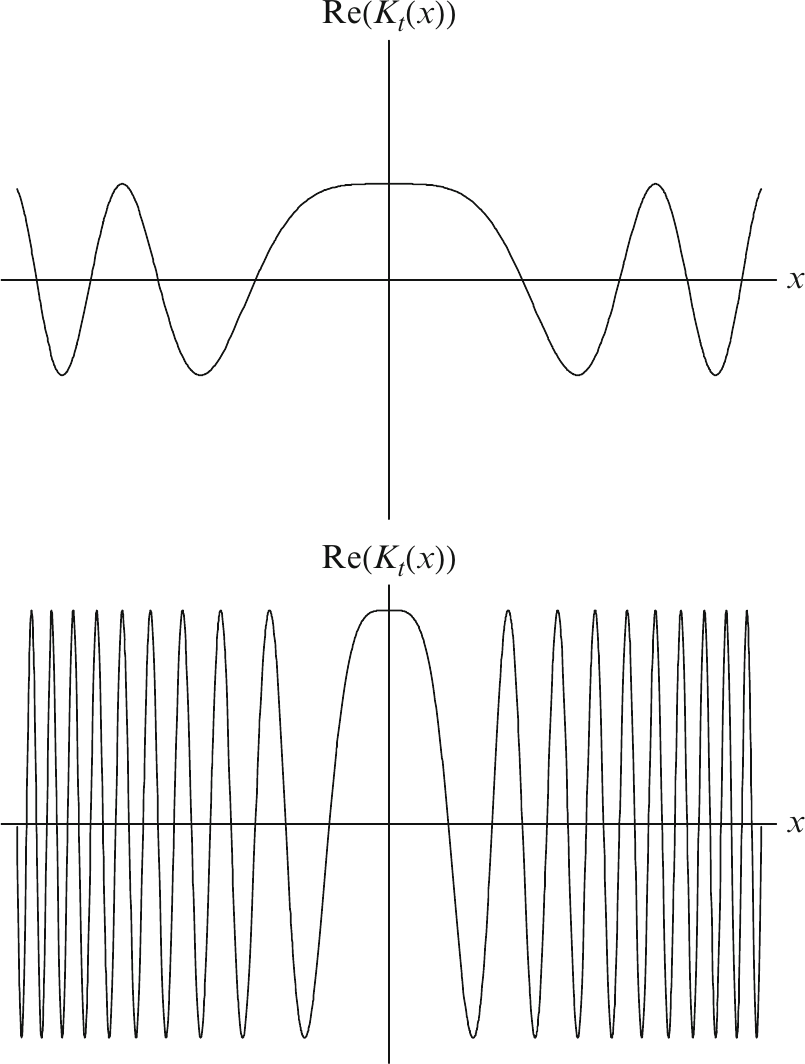
\includegraphics[width=.72\textwidth]{figures/figure-4-1.png}
  \caption{当 \(t=1\)(上图)和 \(t=0.2\)(下图)时,\(K_{t}(x)\) 的实部.}
  \label{fig:free-kernel}
\end{figure}
这里的平方根取实部为正的那个.函数 \(K_{t}\) 称为自由 Schrödinger 方程的基本解(见图~\ref{fig:free-kernel}).直接求导即可验证,\(K_{t}\) 确实满足自由 Schrödinger 方程.

\begin{theorem}[自由方程的卷积公式]\label{thm:free-convolution}
设 \(\psi_{0}\in L^{2}(\mathbb{R})\cap L^{1}(\mathbb{R})\).若 \(\psi(x,t)\) 如式~\eqref{eq:free-fourier-solution} 定义,则对所有 \(t\ne0\),有
\begin{equation}
\psi(x,t)=\sqrt{\frac{m}{2\pi i\hbar t}}
\int_{-\infty}^{\infty}
\exp\left(\frac{im(x-y)^{2}}{2\hbar t}\right)\psi_{0}(y)\,\mathrm{d}y.
\label{eq:free-convolution}
\end{equation}
也就是说,\(\psi(x,t)=(2\pi)^{-1/2}K_{t}*\psi_{0}\),其中 \(K_{t}\) 如式~\eqref{eq:free-kernel}.
\end{theorem}

\begin{proof}
对任意集合 \(E\subset\mathbb{R}\),令 \(\mathbf{1}_{E}\) 表示其示性函数,即在 \(E\) 上为 \(1\),其他地方为 \(0\).对任意正整数 \(n\),\(K_{t}\mathbf{1}_{[-n,n]}\) 属于 \(L^{1}(\mathbb{R})\cap L^{2}(\mathbb{R})\).因此由命题~\ref{app:prop:convolution-fourier},
\[
\mathcal{F}\bigl((K_{t}\mathbf{1}_{[-n,n]})*\psi_{0}\bigr)
=\sqrt{2\pi}\,\mathcal{F}(K_{t}\mathbf{1}_{[-n,n]})\mathcal{F}(\psi_{0}).
\]
由于 \(\psi_{0}\in L^{1}(\mathbb{R})\),容易看出 \(K_{t}\mathbf{1}_{[-n,n]}*\psi_{0}\) 逐点收敛到 \(K_{t}*\psi_{0}\).另一方面,使用练习~\ref{ex:free-gaussian-integral} 中的论证,可以看到 \(\mathcal{F}(K_{t}\mathbf{1}_{[-n,n]})\) 被一个与 \(n\) 无关的常数控制,并逐点收敛到
\[
\frac{1}{\sqrt{2\pi}}\exp\left(-i\frac{\hbar k^{2}}{2m}t\right).
\]
这足以说明式~\eqref{eq:free-convolution-formal} 右端的 Fourier 变换在 \(L^{2}(\mathbb{R})\) 中收敛到
\[
\exp\left(-i\frac{\hbar k^{2}}{2m}t\right)\widehat{\psi}_{0}(k).
\]
由 Plancherel 定理,\(K_{t}\mathbf{1}_{[-n,n]}*\psi_{0}\) 也必须在 \(L^{2}(\mathbb{R})\) 中收敛,而其 \(L^{2}\) 极限必须与逐点极限 \(K_{t}*\psi_{0}\) 一致.对式~\eqref{eq:free-convolution-formal} 两边取极限,就得到所需的 Fourier 变换.

一般来说,要把某个函数称为方程的基本解,还应要求当 \(t\to0\) 时,该函数在分布意义下收敛到 Dirac \(\delta\) 函数(例题~\ref{app:ex:dirac}).由于对每个 \(t\),\(|K_{t}(x)|\) 与 \(x\) 无关,初看之下可能怀疑 \(K_{t}\) 是否有这个性质.另一方面,\(K_{t}(x)\) 除了在 \(x=0\) 附近之外都快速振荡(见图~\ref{fig:free-kernel}).这种振荡使 \(K_{t}(x)\) 与良好函数 \(\psi(x)\) 的积分很小,只有 \(x=0\) 附近的积分部分例外.事实上,由于 \(K_{t}\) 的 Fourier 变换在 \(t\to0\) 时收敛到常函数 \(1/\sqrt{2\pi}\)(这正是形式上取 Dirac \(\delta\) 函数 Fourier 变换所得的结果),不难证明 \(K_{t}\) 确实收敛到 \(\delta\) 函数.细节留给读者.
\end{proof}

\section{波包传播:第一种方法}\label{sec:wave-packet-first}

考虑 \(\mathbb{R}^{1}\) 上的自由 Schrödinger 方程,初始条件 \(\psi_{0}\) 是一个“波包”,即复指数乘以某个将 \(\psi_{0}\) 局部化在空间中的函数.具体取
\begin{equation}
\psi_{0}(x)=e^{ip_{0}x/\hbar}A_{0}(x),
\label{eq:initial-wave-packet}
\end{equation}
其中 \(A_{0}\) 是实的正函数,\(p_{0}\) 是非零实数.(\(p_{0}=0\) 的情形应另行处理.)还假设相对于 \(e^{ip_{0}x/\hbar}\),\(A_{0}\)“变化缓慢”;这意味着在 \(e^{ip_{0}x/\hbar}\) 的许多个周期内,\(A_{0}\) 近似为常数.(稍后会给出“变化缓慢”条件的更精确定义.)因此,如果在只包含几个 \(e^{ip_{0}x/\hbar}\) 周期的小距离尺度上观察 \(\psi_{0}(x)\),它看起来就像常数乘以 \(e^{ip_{0}x/\hbar}\),而后者表示动量为 \(p_{0}\) 的粒子.于是,我们预期 \(\psi_{0}\) 表示一个动量近似等于 \(p_{0}\) 的粒子.

现在尝试用波函数的振幅和相位表示自由 Schrödinger 方程的解.写
\[
\psi(x,t)=A(x,t)e^{i\theta(x,t)},
\]
其中 \(A,\theta\) 是实值函数.把这个表达式代入自由 Schrödinger 方程,并约去每一项中的 \(e^{i\theta(x,t)}\),得到
\begin{equation}
\frac{\partial A}{\partial t}
+iA\frac{\partial\theta}{\partial t}
=\frac{i\hbar}{2m}\frac{\partial^{2}A}{\partial x^{2}}
-\frac{\hbar}{m}\frac{\partial A}{\partial x}\frac{\partial\theta}{\partial x}
-\frac{i\hbar}{2m}A\left(\frac{\partial\theta}{\partial x}\right)^{2}
-\frac{i\hbar}{2m}A\frac{\partial^{2}\theta}{\partial x^{2}}.
\label{eq:amplitude-phase-equation}
\end{equation}
因为 \(A,\theta\) 为实值函数,可以分别令式~\eqref{eq:amplitude-phase-equation} 的实部和虚部相等,得到
\begin{equation}
\frac{\partial A}{\partial t}
=-\frac{\hbar}{m}\frac{\partial A}{\partial x}\frac{\partial\theta}{\partial x}
-\frac{\hbar}{2m}A\frac{\partial^{2}\theta}{\partial x^{2}},
\label{eq:amplitude-equation}
\end{equation}
以及(把虚部除以 \(A\) 后)
\begin{equation}
\frac{\partial\theta}{\partial t}
=\frac{\hbar}{2mA}\frac{\partial^{2}A}{\partial x^{2}}
-\frac{\hbar}{2m}\left(\frac{\partial\theta}{\partial x}\right)^{2}.
\label{eq:phase-equation}
\end{equation}
这个偏微分方程组的任意解都会给出自由 Schrödinger 方程的解 \(\psi(x,t)=A(x,t)e^{i\theta(x,t)}\).

由于我们假设相对于 \(\theta\),\(A\)“变化缓慢”,自然会认为式~\eqref{eq:phase-equation} 右端第一项相对于第二项很小.也就是说,我们把“变化缓慢”理解为
\begin{equation}
\frac{1}{A}\frac{\partial^{2}A}{\partial x^{2}}
\ll\left(\frac{\partial\theta}{\partial x}\right)^{2},
\label{eq:slowly-varying}
\end{equation}
其中 \(\ll\) 表示“远小于”.我们选取在 \(t=0\) 时满足式~\eqref{eq:slowly-varying} 的初始条件,并假定它至少在小的正时间内继续成立.于是(作为一阶近似)可以从式~\eqref{eq:phase-equation} 右端删去第一项,得到简化方程
\begin{equation}
\frac{\partial\theta}{\partial t}
=-\frac{\hbar}{2m}\left(\frac{\partial\theta}{\partial x}\right)^{2}.
\label{eq:approximate-phase}
\end{equation}

现在寻找方程~\eqref{eq:amplitude-equation} 和~\eqref{eq:approximate-phase} 的解,并取与式~\eqref{eq:initial-wave-packet} 对应的初始条件.

\begin{proposition}[波包传播的第一种近似]\label{prop:wave-packet-first}
满足初始条件 \(\theta(x,0)=p_{0}x/\hbar\) 的方程~\eqref{eq:amplitude-equation} 和~\eqref{eq:approximate-phase} 的一个解为
\begin{align}
\theta(x,t)&=\frac{p_{0}}{\hbar}\left(x-\frac{p_{0}}{2m}t\right),\label{eq:wave-packet-phase}\\
A(x,t)&=A_{0}\left(x-\frac{p_{0}}{m}t\right).\label{eq:wave-packet-amplitude}
\end{align}
这给出自由 Schrödinger 方程的近似解
\begin{equation}
\psi(x,t)=A_{0}\left(x-\frac{p_{0}}{m}t\right)
\exp\left[\frac{i}{\hbar}\left(p_{0}x-\frac{p_{0}^{2}}{2m}t\right)\right].
\label{eq:wave-packet-approximation}
\end{equation}
\end{proposition}

从式~\eqref{eq:wave-packet-phase} 和~\eqref{eq:wave-packet-amplitude} 可以看出,如果“变化缓慢”条件~\eqref{eq:slowly-varying} 在时刻 \(0\) 成立,那么在我们的近似解中,它会对所有正时间继续成立.

\begin{proof}
虽然式~\eqref{eq:approximate-phase} 是非线性方程,但对初始条件 \(\theta(x,0)=p_{0}x/\hbar\),可以找到简单的解
\[
\theta(x,t)=\frac{p_{0}x}{\hbar}-\frac{p_{0}^{2}}{2m\hbar}t
=\frac{p_{0}}{\hbar}\left(x-\frac{p_{0}}{2m}t\right).
\]
由于 \(\partial\theta/\partial x=p_{0}/\hbar\),且 \(\partial^{2}\theta/\partial x^{2}=0\),将其代回式~\eqref{eq:amplitude-equation},得到
\[
\frac{\partial A}{\partial t}
=-\frac{p_{0}}{m}\frac{\partial A}{\partial x}.
\]
这个线性方程以 \(A(x,0)=A_{0}(x)\) 为初始条件的(推测唯一)解为
\[
A(x,t)=A_{0}\left(x-\frac{p_{0}}{m}t\right),
\]
命题得证.
\end{proof}

我们希望,在 \(A_{0}\) 相对于初始相位 \(\theta_{0}(x)=p_{0}x/\hbar\) 变化缓慢的前提下,式~\eqref{eq:wave-packet-approximation} 是原方程~\eqref{eq:amplitude-equation} 和~\eqref{eq:phase-equation} 解的良好近似.不过,直接估计式~\eqref{eq:amplitude-equation}--\eqref{eq:phase-equation} 的解彼此偏离的速度并不容易.因此,我们把近似误差的估计留到下一节;在那里将用不同方法得到同一个近似解.

注意,形如 \(f(x,t)=\phi(x-vt)\) 的函数以恒定速度 \(v\) 向右运动(如果 \(v<0\),当然表示向左运动).振幅 \(A(x,t)\) 和相位因子 \(e^{i\theta(x,t)}\) 都具有这种形式,但对应两个不同的速度.

\begin{conclusion}[群速度与相速度]\label{con:group-phase-velocity}
在自由 Schrödinger 方程的近似解~\eqref{eq:wave-packet-approximation} 中,振幅 \(A(x,t)\) 以速度 \(p_{0}/m\) 运动,而相位 \(\theta(x,t)\) 以速度 \(p_{0}/(2m)\) 运动.这两个速度分别称为群速度和相速度:
\[
\text{相速度}=\frac{p_{0}}{2m},
\qquad
\text{群速度}=\frac{p_{0}}{m}.
\]
\end{conclusion}

相速度公式与前面第~\ref{sec:free-fourier} 节给出的公式一致;那里相速度是自由 Schrödinger 方程纯指数解的传播速度.事实上,取 \(A_{0}\equiv1\),式~\eqref{eq:slowly-varying} 左端恒等于零,于是方程~\eqref{eq:amplitude-equation} 和~\eqref{eq:phase-equation} 的解也确实是原方程的解.

哪个速度是粒子的“真实”速度？答案是群速度.毕竟,粒子位置的概率分布由波函数的振幅决定,而不受相位影响.振幅决定了粒子在哪里(在可确定的程度内).因此,粒子的真实速度应是振幅传播的速度.图~\ref{fig:free-wave-packet} 展示了波包实部的传播,并用阴影区域标出一个峰的运动.相速度决定 \(\psi\) 实部中各个峰的运动速度,而群速度决定整个波包的运动速度.由于我们跟踪的峰明显落后于整个波包的运动,可以看出相速度小于群速度.

\begin{figure}[htbp]
  \centering
  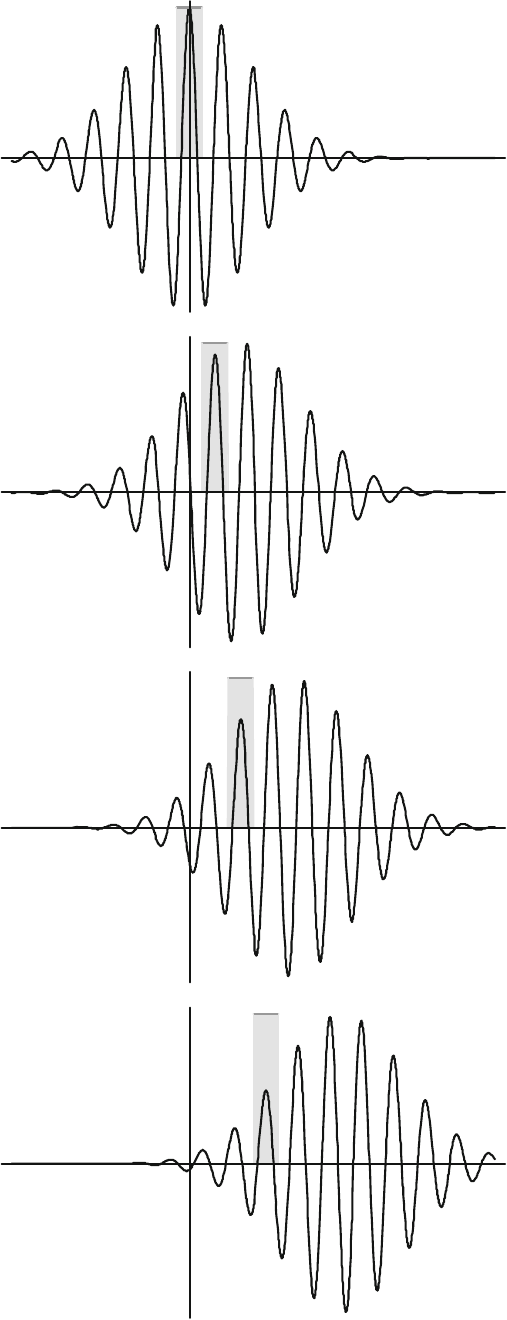
\includegraphics[width=.48\textwidth]{figures/figure-4-2.png}
  \caption{\(\operatorname{Re}[\psi]\) 的传播,其中阴影部分标出了单个峰的运动.}
  \label{fig:free-wave-packet}
\end{figure}

我们应当预期,方程~\eqref{eq:amplitude-equation} 和~\eqref{eq:approximate-phase} 的解会随时间缓慢偏离自由 Schrödinger 方程~\eqref{eq:amplitude-equation} 和~\eqref{eq:phase-equation} 的解.经过足够长时间,近似解与真实解之间可能有明显差异.这一预期将在第~\ref{sec:wave-packet-spread} 节得到确认;那里将研究波包扩散,而这一现象在当前近似中看不到.

\section{波包传播:第二种方法}\label{sec:wave-packet-second}

我们已经看到,自由 Schrödinger 方程的一般解可以通过 Fourier 变换写成
\begin{equation}
\psi(x,t)=\frac{1}{\sqrt{2\pi}}\int_{-\infty}^{\infty}
\widehat{\psi}_{0}(k)\exp[i(kx-\omega(k)t)]\,\mathrm{d}k,
\label{eq:free-fourier-general}
\end{equation}
其中
\[
\omega(k)=\frac{\hbar k^{2}}{2m}.
\]
假设 \(\psi_{0}\) 的近似动量为 \(p_{0}\).于是预期 \(\widehat{\psi}_{0}(k)\) 集中在 \(k_{0}:=p_{0}/\hbar\) 附近.如果确实如此,那么只有接近 \(k_{0}\) 的 \(k\) 值重要.对接近 \(k_{0}\) 的 \(k\),使用一阶 Taylor 展开
\begin{equation}
\omega(k)\approx\omega(k_{0})+\omega'(k_{0})(k-k_{0}).
\label{eq:dispersion-linearization}
\end{equation}

把式~\eqref{eq:dispersion-linearization} 代入式~\eqref{eq:free-fourier-general},两个与 \(k\) 无关的因子可以移到积分号外,得到
\begin{align}
\psi(x,t)
&\approx\frac{1}{\sqrt{2\pi}}e^{i\omega'(k_{0})k_{0}t}e^{-i\omega(k_{0})t}
\int_{-\infty}^{\infty}\widehat{\psi}_{0}(k)
\exp[i k(x-\omega'(k_{0})t)]\,\mathrm{d}k\notag\\
&=e^{i\omega'(k_{0})k_{0}t}e^{-i\omega(k_{0})t}
\psi_{0}(x-\omega'(k_{0})t).
\label{eq:wave-packet-fourier-approx}
\end{align}
注意,\(\psi_{0}(x-\omega'(k_{0})t)\) 前的因子只是与 \(x\) 无关的常数.这些常数不影响系统的“状态”,因为我们已经约定,量子 Hilbert 空间中相差一个常数的两个向量代表同一物理状态.忽略这些常数,剩下的因子 \(\psi_{0}(x-\omega'(k_{0})t)\) 正是以速度 \(\omega'(k_{0})\) 向右平移的函数.因此,波包运动的(近似)速度为
       \[
\text{速度}\approx\omega'(k_{0})
=\frac{\hbar k_{0}}{m}
=\frac{p_{0}}{m}.
\]

考虑 \(\psi_{0}(x)=e^{ik_{0}x}A_{0}(x)\) 的特殊情形,其中 \(A_{0}\) 实且为正.那么式~\eqref{eq:wave-packet-fourier-approx} 变为
\[
e^{i\omega'(k_{0})k_{0}t}e^{-i\omega(k_{0})t}
e^{ik_{0}(x-\omega'(k_{0})t)}
A_{0}(x-\omega'(k_{0})t).
\]
约去指数中包含 \(\omega'(k_{0})k_{0}t\) 的项,得到
\[
\psi(x,t)\approx e^{i(k_{0}x-\omega(k_{0})t)}
A_{0}(x-\omega'(k_{0})t).
\]
回忆 \(p_{0}=\hbar k_{0}\),代入 \(\omega\) 的公式可知,这个 \(\psi(x,t)\) 的近似正是我们在命题~\ref{prop:wave-packet-first} 中通过另一种方法得到的近似.

与第~\ref{sec:wave-packet-first} 节一样,自由 Schrödinger 方程的纯指数解传播速度 \(\omega(k_{0})/k_{0}=\hbar k_{0}/(2m)\) 与整个波包的传播速度不同.由式~\eqref{eq:wave-packet-fourier-approx} 可见,波包以 \(\omega'(k_{0})=\hbar k_{0}/m\) 的速度传播.总结如下.

\begin{proposition}[群速度与相速度的 Fourier 观点]\label{prop:group-phase-velocity}
自由 Schrödinger 方程的纯指数解传播的速度为
\[
\text{相速度}=\frac{\omega(k_{0})}{k_{0}}
=\frac{\hbar k_{0}}{2m}
=\frac{p_{0}}{2m}.
\]
相比之下,波包传播的(近似)速度为
\[
\text{群速度}
=\left.\frac{\mathrm{d}\omega}{\mathrm{d}k}\right|_{k=k_{0}}
=\frac{\hbar k_{0}}{m}
=\frac{p_{0}}{m}.
\]
\end{proposition}

第~\ref{sec:wave-packet-first} 节的方法不容易直接给出近似误差的大小估计.不过,在本节中可以通过比较精确解与近似解的 Fourier 变换来估计误差.为此定义
\begin{equation}
\kappa:=\left(\int_{-\infty}^{\infty}
|\widehat{\psi}_{0}(k)|^{2}(k-k_{0})^{4}\,\mathrm{d}k\right)^{1/4}.
\label{eq:wave-packet-concentration}
\end{equation}
\(\kappa\) 大致是 \(\widehat{\psi}_{0}(k)\) 大部分集中所在的、以 \(k_{0}\) 为中心的区间宽度的一半.例如,如果 \(\widehat{\psi}_{0}\) 支集包含在 \([k_{0}-\varepsilon,k_{0}+\varepsilon]\) 中,并且 \(\psi_{0}\)(因而 \(\widehat{\psi}_{0}\))是单位向量,则 \(\kappa\le\varepsilon\).更常见的集中度量会用 \((k-k_{0})^{2}\) 替换四次幂,并用平方根而非四次根.不过,式~\eqref{eq:wave-packet-concentration} 中的“四次”度量正是本节误差估计中出现的量.

\begin{proposition}[波包近似的误差估计]\label{prop:wave-packet-error}
设 \(\psi(x,t)\) 是初始条件为 \(\psi_{0}\) 的自由 Schrödinger 方程精确解,\(\phi(x,t)\) 是式~\eqref{eq:wave-packet-fourier-approx} 右端给出的近似解,则有 \(L^{2}\) 估计
\begin{equation}
\|\psi(x,t)-\phi(x,t)\|_{L^{2}(\mathbb{R})}
\le\frac{|t|\hbar\kappa^{2}}{2m}
=|t|\,\omega(\kappa),
\label{eq:wave-packet-error}
\end{equation}
其中 \(L^{2}\) 范数固定 \(t\) 关于 \(x\) 取,\(\omega\) 由式~\eqref{eq:free-dispersion} 定义.
\end{proposition}

式~\eqref{eq:wave-packet-error} 意味着,只要
\[
|t|\ll\frac{1}{\omega(\kappa)},
\]
\(L^{2}\) 意义下的误差就会很小.如果 \(\kappa\ll k_{0}\),那么 \(1/\omega(\kappa)\) 会远大于 \(1/\omega(k_{0})\).这意味着真实解和近似解开始明显偏离的时间尺度,远长于近似解振荡的时间尺度.

\begin{proof}
记 \(\widehat{\psi}(k,t)\) 和 \(\widehat{\phi}(k,t)\) 为固定 \(t\) 关于 \(x\) 的 Fourier 变换.由式~\eqref{eq:free-fourier-general} 可读出
\[
\widehat{\psi}(k,t)=e^{-i\omega(k)t}\widehat{\psi}_{0}(k).
\]
另一方面,\(\widehat{\phi}(k,t)\) 由 \(\widehat{\psi}(k,t)\) 将 \(\omega(k)\) 替换为式~\eqref{eq:dispersion-linearization} 右端得到.直接计算可得
\[
\omega(k)-\bigl(\omega(k_{0})+\omega'(k_{0})(k-k_{0})\bigr)
=\frac{\hbar}{2m}(k-k_{0})^{2}.
\]
利用初等估计 \(|e^{i\theta}-e^{i\varphi}|\le|\theta-\varphi|\),得到
\[
|\widehat{\psi}(k,t)-\widehat{\phi}(k,t)|
\le\frac{|t|\hbar}{2m}(k-k_{0})^{2}|\widehat{\psi}_{0}(k)|.
\]
于是由 Plancherel 定理和 \(\kappa\) 的定义得到式~\eqref{eq:wave-packet-error}.
\end{proof}

\section{波包的扩散}\label{sec:wave-packet-spread}

我们用粒子位置的不确定度 \(\Delta_{\psi}X\)(定义~\ref{def:quantum-uncertainty})作为 \(\psi(x)\) 这个函数“宽度”的度量.在前两节所考虑的近似层次上,自由粒子的位置不确定度与时间无关.毕竟,在近似解~\eqref{eq:wave-packet-approximation} 中,波函数的振幅只以群速度向右平移,而形状不变.不过,更精确的计算表明,经过足够长时间后,波包会在空间中扩散.(练习~\ref{ex:free-spread-rate} 可以帮助理解扩散发生的时间尺度.)

利用第~3 章的命题~\ref{prop:expectation-evolution},无需求出完整的 Schrödinger 方程解,就可以计算粒子位置不确定度的时间演化.对自由粒子,Hamilton 算子就是 \(P^{2}/(2m)\),它与 \(P\) 对易.因此,粒子的动量期望值、不确定度(事实上包括动量的整个概率分布)都与时间无关.另一方面,要计算 \(\langle X\rangle\) 和 \(\langle X^{2}\rangle\) 的时间依赖,可以使用命题~\ref{prop:expectation-evolution} 以及对易关系 \([X,P]=i\hbar I\)(命题~\ref{prop:canonical-commutation-one}).

\begin{proposition}[自由粒子的波包扩散]\label{prop:free-wave-spread}
若波函数 \(\psi(x,t)\) 按照 \(\mathbb{R}^{1}\) 上的自由 Schrödinger 方程演化,则
\begin{align}
\langle X\rangle_{\psi(t)}
&=\langle X\rangle_{\psi_{0}}+\frac{t}{m}\langle P\rangle_{\psi_{0}},\label{eq:free-position-time}\\
\langle X^{2}\rangle_{\psi(t)}
&=\langle X^{2}\rangle_{\psi_{0}}
+\frac{t}{m}\langle XP+PX\rangle_{\psi_{0}}
+\frac{t^{2}}{m^{2}}\langle P^{2}\rangle_{\psi_{0}}.\label{eq:free-position-square-time}
\end{align}
从而
\begin{equation}
(\Delta_{\psi(t)}X)^{2}
=(\Delta_{\psi_{0}}X)^{2}
+\frac{t}{m}\left(\langle XP+PX\rangle_{\psi_{0}}
-2\langle X\rangle_{\psi_{0}}\langle P\rangle_{\psi_{0}}\right)
+\frac{t^{2}}{m^{2}}(\Delta_{\psi_{0}}P)^{2}.
\label{eq:free-position-uncertainty}
\end{equation}
\end{proposition}

对于 \(L^{2}(\mathbb{R})\) 中的单位向量 \(\psi_{0}\),动量不确定度 \(\Delta_{\psi_{0}}P\) 不可能为零,因为不确定度为零意味着 \(\psi_{0}\) 是动量算子的特征向量,而 \(P\) 的特征向量是形如 \(e^{ikx}\) 的函数,它们不属于 \(L^{2}(\mathbb{R})\).因此,式~\eqref{eq:free-position-uncertainty} 中 \(t^{2}\) 项的系数永不为零,从而当 \(t\to\infty\) 时,\(\Delta_{\psi(t)}X\to\infty\).

\begin{proof}
计算得
\[
[P^{2},X]=P[P,X]+[P,X]P=-2i\hbar P.
\]
因此(正如我们在第~\ref{subsec:expected-position-momentum} 节已经指出的),
\[
\frac{\mathrm{d}}{\mathrm{d}t}\langle X\rangle_{\psi(t)}
=\left\langle\frac{i}{\hbar}(-2i\hbar P)\right\rangle_{\psi(t)}
=\frac{\langle P\rangle_{\psi(t)}}{m}
=\frac{\langle P\rangle_{\psi_{0}}}{m},
\]
其中最后一个等号使用了动量期望值与时间无关这一事实.由于 \(\langle X\rangle_{\psi(t)}\) 的导数是常数,它关于 \(t\) 是线性的,于是得到命题中的第一个结果.

另一方面,直接计算可得
\[
[P^{2},X^{2}]
=-2i\hbar(PX+XP),
\]
以及
\[
[P^{2},PX+XP]=-4i\hbar P^{2}.
\]
因此
\[
\frac{\mathrm{d}}{\mathrm{d}t}\langle X^{2}\rangle_{\psi(t)}
=\frac{1}{m}\langle XP+PX\rangle_{\psi(t)},
\]
并且
\[
\frac{\mathrm{d}^{2}}{\mathrm{d}t^{2}}\langle X^{2}\rangle_{\psi(t)}
=\frac{2}{m^{2}}\langle P^{2}\rangle_{\psi(t)}
=\frac{2}{m^{2}}\langle P^{2}\rangle_{\psi_{0}}.
\]
由于 \(\langle X^{2}\rangle_{\psi(t)}\) 的二阶导数与时间无关,它关于 \(t\) 是二次多项式;其系数由 \(t=0\) 时 \(\langle X\rangle_{\psi(t)}\) 的值以及前两个时间导数确定.这给出式~\eqref{eq:free-position-square-time}.最后一个结果直接计算即可得到.
\end{proof}

\section{练习}\label{sec:chapter4-exercises}

\begin{exercise}\label{ex:free-weak-solution}
局部可积函数 \(\psi(x,t)\) 在弱(或分布)意义下满足自由 Schrödinger 方程,是指对每个光滑紧支集函数 \(\chi\),都有
\begin{equation}
\int_{\mathbb{R}^{2}}\psi(x,t)\left(\frac{\partial\chi}{\partial t}
+\frac{i\hbar}{2m}\frac{\partial^{2}\chi}{\partial x^{2}}\right)\,\mathrm{d}x\,\mathrm{d}t=0.
\label{eq:free-weak-equation}
\end{equation}
(式~\eqref{eq:free-weak-equation} 的得到方式是,假定 \(\partial\psi/\partial t-(i\hbar/2m)\partial^{2}\psi/\partial x^{2}=0\),再与 \(\chi(x,t)\) 相乘并形式地分部积分.)
\begin{enumerate}
\item 证明,如果 \(\psi(x,t)\) 关于 \(x,t\) 光滑,则它在逐点意义下满足自由 Schrödinger 方程,当且仅当它在弱意义下满足自由 Schrödinger 方程.提示:命题~\ref{app:prop:distribution-constant} 可能有用.
\item 对任意 \(\psi_{0}\in L^{2}(\mathbb{R})\),按定义~\ref{def:free-l2-evolution} 定义 \(\psi(x,t)\).证明 \(\psi\) 在弱意义下满足自由 Schrödinger 方程.先证明对每个 \(A\),函数
\[
\psi_{A}(x,t)=\frac{1}{\sqrt{2\pi}}\int_{-A}^{A}
\widehat{\psi}_{0}(k)e^{i(kx-\omega(k)t)}\,\mathrm{d}k
\]
在弱意义下满足自由 Schrödinger 方程.
\end{enumerate}
\end{exercise}

\begin{exercise}\label{ex:free-gaussian-integral}
\begin{enumerate}
\item 证明,对任意 \(\operatorname{Re}(a)>0\) 的复数 \(a\),有
\[
\int_{-\infty}^{\infty}e^{-x^{2}/(2a)}\,\mathrm{d}x
=\iint_{\mathbb{R}^{2}}e^{-(x^{2}+y^{2})/(2a)}\,\mathrm{d}x\,\mathrm{d}y
=2\pi a,
\]
其中 \(\mathbb{R}^{2}\) 上的积分可用极坐标计算.推出(平方根取实部为正)
\[
\int_{-\infty}^{\infty}e^{-x^{2}/(2a)}\,\mathrm{d}x=\sqrt{2\pi a}.
\]
\item 证明,对任意 \(A,B>0\) 以及任意非零复数 \(a\),有
\[
\int_{A}^{B}e^{-x^{2}/(2a)}\,\mathrm{d}x
=\left.-\frac{a}{x}e^{-x^{2}/(2a)}\right|_{A}^{B}
-a\int_{A}^{B}\frac{1}{x^{2}}e^{-x^{2}/(2a)}\,\mathrm{d}x.
\]
利用它证明,当非零 \(a\) 满足 \(\operatorname{Re}(a)\ge0\) 时,只要把积分理解为广义积分(即取 \([-A,A]\) 上积分并令 \(A\to\infty\) 的极限),式~\eqref{eq:free-kernel} 中的积分收敛.
\item 证明 (a) 的结论对非零且 \(\operatorname{Re}(a)=0\) 的 \(a\) 也成立.提示:给定 \(\beta\ne0\),证明当 \(A\) 很大时,从 \(A\) 到 \(\infty\) 的 \(\exp[-x^{2}/(2(\alpha+i\beta))]\) 积分,对 \(\alpha\in[0,1]\) 一致地很小.
\item 证明(积分理解为广义积分,平方根取实部为正)
\[
\frac{1}{2\pi}\int_{-\infty}^{\infty}e^{ikx}e^{-it\hbar k^{2}/(2m)}\,\mathrm{d}k
=\sqrt{\frac{m}{2\pi i\hbar t}}e^{imx^{2}/(2t\hbar)}.
\]
\end{enumerate}
\end{exercise}

\begin{exercise}\label{ex:convolution-smooth}
设 \(\phi\) 是 Schwartz 函数(定义~\ref{app:def:schwartz}),\(\psi\in L^{2}(\mathbb{R})\).证明卷积 \(\phi*\psi\) 是光滑函数(无穷可微).
\end{exercise}

\begin{exercise}\label{ex:heat-equation}
考虑函数 \(\psi(x,t)\) 的热方程
\[
\frac{\partial\psi}{\partial t}
=\alpha\frac{\partial^{2}\psi}{\partial x^{2}},
\]
其中 \(\alpha\) 是常数,初始条件为 \(\psi(x,0)=\psi_{0}(x)\).
\begin{enumerate}
\item 假设对每个 \(t\),\(\psi(x,t)\) 关于 \(x\) 足够良好.推导热方程解关于 \(x\) 的 Fourier 变换 \(\widehat{\psi}(k,t)\) 所满足的微分方程,并求出满足 \(\widehat{\psi}(k,0)=\widehat{\psi}_{0}(k)\) 的解.
\item 把热方程的解表示为 \(\psi_{0}\) 与热方程某个“基本解”的卷积.
\end{enumerate}
\begin{note}
正如第~20 章将讨论的,热方程可以看成自由 Schrödinger 方程的某种“虚时间”版本.
\end{note}
\end{exercise}

\begin{exercise}\label{ex:gaussian-wave-packet}
设自由 Schrödinger 方程的初始相位为 \(\theta_{0}(x)=p_{0}x/\hbar\),初始振幅为 \(A_{0}(x)\),如式~\eqref{eq:initial-wave-packet}.再假设
\[
A_{0}(x)=\exp\left(-\frac{1}{2}\left(\frac{x-x_{0}}{L}\right)^{2}\right).
\]
注意,\(A_{0}\) 以 \(x_{0}\) 为中心,参数 \(L\) 衡量初始波包在空间中的宽度.具有这种 \(A_{0}\) 的 \(\psi_{0}(x)=e^{ip_{0}x/\hbar}A_{0}(x)\) 称为 Gaussian 波包.计算
\[
\left(\frac{\partial\theta_{0}}{\partial x}\right)^{-2}
\left(\frac{1}{A_{0}}\frac{\partial^{2}A_{0}}{\partial x^{2}}\right).
\]
假设 \(\hbar\) 相对于 \(Lp_{0}\) 很小,证明除非在初始波包非常小的点处,否则上式很小.
\begin{note}
这说明对 Gaussian 波包而言,“变化缓慢”假设~\eqref{eq:slowly-varying} 是合理的.
\end{note}
\end{exercise}

\begin{exercise}\label{ex:klein-gordon}
Klein--Gordon 方程是 Schrödinger 方程的一种拟议的相对论替代理论:
\[
\frac{1}{c^{2}}\frac{\partial^{2}\psi}{\partial t^{2}}
=\frac{\partial^{2}\psi}{\partial x^{2}}-\frac{m^{2}c^{2}}{\hbar^{2}}\psi,
\]
其中 \(m>0\) 是粒子质量,\(c\) 是光速.
\begin{enumerate}
\item 求 Klein--Gordon 方程的色散关系,即找出使 \(\exp[i(kx-\omega(k)t)]\) 成为方程解的 \(\omega(k)\).
\item 证明相速度 \(\omega(k)/k\) 满足 \(|\omega(k)/k|>c\),群速度 \(\mathrm{d}\omega(k)/\mathrm{d}k\) 满足 \(|\mathrm{d}\omega/\mathrm{d}k|<c\),并且
\[
(\text{相速度})(\text{群速度})=c^{2}.
\]
\end{enumerate}
\begin{note}
由于 Klein--Gordon 方程关于时间是二阶的,对每个 \(k\) 有两个可能的 \(\omega(k)\),一个为正,一个为负.(b) 的结论对 \(\omega(k)\) 的两支都成立.
\end{note}
\end{exercise}

\begin{exercise}\label{ex:free-spread-rate}
考虑按自由 Schrödinger 方程演化的波函数 \(\psi(t)\) 的位置不确定度 \(\Delta_{\psi(t)}X\).证明对所有 \(t\),
\begin{equation}
\left|\frac{\mathrm{d}}{\mathrm{d}t}\Delta_{\psi(t)}X\right|
\le\frac{\Delta_{\psi_{0}}P}{m},
\label{eq:free-spread-bound}
\end{equation}
并证明
\[
\lim_{t\to+\infty}\frac{\mathrm{d}}{\mathrm{d}t}\Delta_{\psi(t)}X
=\frac{\Delta_{\psi_{0}}P}{m}.
\]
\begin{note}
相比之下,
\[
\frac{\mathrm{d}}{\mathrm{d}t}\langle X\rangle_{\psi(t)}
=\frac{\langle P\rangle_{\psi_{0}}}{m}.
\]
如果 \(\widehat{\psi}_{0}(k)\) 集中在非零数 \(k_{0}=p_{0}/\hbar\) 附近的一个足够小的区域,那么 \(\Delta_{\psi_{0}}P\) 会远小于 \(\langle P\rangle_{\psi_{0}}\).比较式~\eqref{eq:free-spread-bound} 与上述式子可知,此时波包扩散的速率相对于波包运动的速率很小.
\end{note}
\end{exercise}
